


% Header, overrides base

    % Make sure that the sphinx doc style knows who it inherits from.
    \def\sphinxdocclass{article}

    % Declare the document class
    \documentclass[letterpaper,10pt,english]{/Library/Python/2.7/site-packages/sphinx/texinputs/sphinxhowto}

    % Imports
    \usepackage[utf8]{inputenc}
    \DeclareUnicodeCharacter{00A0}{\\nobreakspace}
    \usepackage[T1]{fontenc}
    \usepackage{babel}
    \usepackage{times}
    \usepackage{import}
    \usepackage[Bjarne]{/Library/Python/2.7/site-packages/sphinx/texinputs/fncychap}
    \usepackage{longtable}
    \usepackage{/Library/Python/2.7/site-packages/sphinx/texinputs/sphinx}
    \usepackage{multirow}

    \usepackage{amsmath}
    \usepackage{amssymb}
    \usepackage{ucs}
    \usepackage{enumerate}

    % Used to make the Input/Output rules follow around the contents.
    \usepackage{needspace}

    % Pygments requirements
    \usepackage{fancyvrb}
    \usepackage{color}
    % ansi colors additions
    \definecolor{darkgreen}{rgb}{.12,.54,.11}
    \definecolor{lightgray}{gray}{.95}
    \definecolor{brown}{rgb}{0.54,0.27,0.07}
    \definecolor{purple}{rgb}{0.5,0.0,0.5}
    \definecolor{darkgray}{gray}{0.25}
    \definecolor{lightred}{rgb}{1.0,0.39,0.28}
    \definecolor{lightgreen}{rgb}{0.48,0.99,0.0}
    \definecolor{lightblue}{rgb}{0.53,0.81,0.92}
    \definecolor{lightpurple}{rgb}{0.87,0.63,0.87}
    \definecolor{lightcyan}{rgb}{0.5,1.0,0.83}

    % Needed to box output/input
    \usepackage{tikz}
        \usetikzlibrary{calc,arrows,shadows}
    \usepackage[framemethod=tikz]{mdframed}

    \usepackage{alltt}

    % Used to load and display graphics
    \usepackage{graphicx}
    \graphicspath{ {figs/} }
    \usepackage[Export]{adjustbox} % To resize

    % used so that images for notebooks which have spaces in the name can still be included
    \usepackage{grffile}


    % For formatting output while also word wrapping.
    \usepackage{listings}
    \lstset{breaklines=true}
    \lstset{basicstyle=\small\ttfamily}
    \def\smaller{\fontsize{9.5pt}{9.5pt}\selectfont}

    %Pygments definitions
    
\makeatletter
\def\PY@reset{\let\PY@it=\relax \let\PY@bf=\relax%
    \let\PY@ul=\relax \let\PY@tc=\relax%
    \let\PY@bc=\relax \let\PY@ff=\relax}
\def\PY@tok#1{\csname PY@tok@#1\endcsname}
\def\PY@toks#1+{\ifx\relax#1\empty\else%
    \PY@tok{#1}\expandafter\PY@toks\fi}
\def\PY@do#1{\PY@bc{\PY@tc{\PY@ul{%
    \PY@it{\PY@bf{\PY@ff{#1}}}}}}}
\def\PY#1#2{\PY@reset\PY@toks#1+\relax+\PY@do{#2}}

\expandafter\def\csname PY@tok@gd\endcsname{\def\PY@tc##1{\textcolor[rgb]{0.63,0.00,0.00}{##1}}}
\expandafter\def\csname PY@tok@gu\endcsname{\let\PY@bf=\textbf\def\PY@tc##1{\textcolor[rgb]{0.50,0.00,0.50}{##1}}}
\expandafter\def\csname PY@tok@gt\endcsname{\def\PY@tc##1{\textcolor[rgb]{0.00,0.27,0.87}{##1}}}
\expandafter\def\csname PY@tok@gs\endcsname{\let\PY@bf=\textbf}
\expandafter\def\csname PY@tok@gr\endcsname{\def\PY@tc##1{\textcolor[rgb]{1.00,0.00,0.00}{##1}}}
\expandafter\def\csname PY@tok@cm\endcsname{\let\PY@it=\textit\def\PY@tc##1{\textcolor[rgb]{0.25,0.50,0.50}{##1}}}
\expandafter\def\csname PY@tok@vg\endcsname{\def\PY@tc##1{\textcolor[rgb]{0.10,0.09,0.49}{##1}}}
\expandafter\def\csname PY@tok@m\endcsname{\def\PY@tc##1{\textcolor[rgb]{0.40,0.40,0.40}{##1}}}
\expandafter\def\csname PY@tok@mh\endcsname{\def\PY@tc##1{\textcolor[rgb]{0.40,0.40,0.40}{##1}}}
\expandafter\def\csname PY@tok@go\endcsname{\def\PY@tc##1{\textcolor[rgb]{0.53,0.53,0.53}{##1}}}
\expandafter\def\csname PY@tok@ge\endcsname{\let\PY@it=\textit}
\expandafter\def\csname PY@tok@vc\endcsname{\def\PY@tc##1{\textcolor[rgb]{0.10,0.09,0.49}{##1}}}
\expandafter\def\csname PY@tok@il\endcsname{\def\PY@tc##1{\textcolor[rgb]{0.40,0.40,0.40}{##1}}}
\expandafter\def\csname PY@tok@cs\endcsname{\let\PY@it=\textit\def\PY@tc##1{\textcolor[rgb]{0.25,0.50,0.50}{##1}}}
\expandafter\def\csname PY@tok@cp\endcsname{\def\PY@tc##1{\textcolor[rgb]{0.74,0.48,0.00}{##1}}}
\expandafter\def\csname PY@tok@gi\endcsname{\def\PY@tc##1{\textcolor[rgb]{0.00,0.63,0.00}{##1}}}
\expandafter\def\csname PY@tok@gh\endcsname{\let\PY@bf=\textbf\def\PY@tc##1{\textcolor[rgb]{0.00,0.00,0.50}{##1}}}
\expandafter\def\csname PY@tok@ni\endcsname{\let\PY@bf=\textbf\def\PY@tc##1{\textcolor[rgb]{0.60,0.60,0.60}{##1}}}
\expandafter\def\csname PY@tok@nl\endcsname{\def\PY@tc##1{\textcolor[rgb]{0.63,0.63,0.00}{##1}}}
\expandafter\def\csname PY@tok@nn\endcsname{\let\PY@bf=\textbf\def\PY@tc##1{\textcolor[rgb]{0.00,0.00,1.00}{##1}}}
\expandafter\def\csname PY@tok@no\endcsname{\def\PY@tc##1{\textcolor[rgb]{0.53,0.00,0.00}{##1}}}
\expandafter\def\csname PY@tok@na\endcsname{\def\PY@tc##1{\textcolor[rgb]{0.49,0.56,0.16}{##1}}}
\expandafter\def\csname PY@tok@nb\endcsname{\def\PY@tc##1{\textcolor[rgb]{0.00,0.50,0.00}{##1}}}
\expandafter\def\csname PY@tok@nc\endcsname{\let\PY@bf=\textbf\def\PY@tc##1{\textcolor[rgb]{0.00,0.00,1.00}{##1}}}
\expandafter\def\csname PY@tok@nd\endcsname{\def\PY@tc##1{\textcolor[rgb]{0.67,0.13,1.00}{##1}}}
\expandafter\def\csname PY@tok@ne\endcsname{\let\PY@bf=\textbf\def\PY@tc##1{\textcolor[rgb]{0.82,0.25,0.23}{##1}}}
\expandafter\def\csname PY@tok@nf\endcsname{\def\PY@tc##1{\textcolor[rgb]{0.00,0.00,1.00}{##1}}}
\expandafter\def\csname PY@tok@si\endcsname{\let\PY@bf=\textbf\def\PY@tc##1{\textcolor[rgb]{0.73,0.40,0.53}{##1}}}
\expandafter\def\csname PY@tok@s2\endcsname{\def\PY@tc##1{\textcolor[rgb]{0.73,0.13,0.13}{##1}}}
\expandafter\def\csname PY@tok@vi\endcsname{\def\PY@tc##1{\textcolor[rgb]{0.10,0.09,0.49}{##1}}}
\expandafter\def\csname PY@tok@nt\endcsname{\let\PY@bf=\textbf\def\PY@tc##1{\textcolor[rgb]{0.00,0.50,0.00}{##1}}}
\expandafter\def\csname PY@tok@nv\endcsname{\def\PY@tc##1{\textcolor[rgb]{0.10,0.09,0.49}{##1}}}
\expandafter\def\csname PY@tok@s1\endcsname{\def\PY@tc##1{\textcolor[rgb]{0.73,0.13,0.13}{##1}}}
\expandafter\def\csname PY@tok@sh\endcsname{\def\PY@tc##1{\textcolor[rgb]{0.73,0.13,0.13}{##1}}}
\expandafter\def\csname PY@tok@sc\endcsname{\def\PY@tc##1{\textcolor[rgb]{0.73,0.13,0.13}{##1}}}
\expandafter\def\csname PY@tok@sx\endcsname{\def\PY@tc##1{\textcolor[rgb]{0.00,0.50,0.00}{##1}}}
\expandafter\def\csname PY@tok@bp\endcsname{\def\PY@tc##1{\textcolor[rgb]{0.00,0.50,0.00}{##1}}}
\expandafter\def\csname PY@tok@c1\endcsname{\let\PY@it=\textit\def\PY@tc##1{\textcolor[rgb]{0.25,0.50,0.50}{##1}}}
\expandafter\def\csname PY@tok@kc\endcsname{\let\PY@bf=\textbf\def\PY@tc##1{\textcolor[rgb]{0.00,0.50,0.00}{##1}}}
\expandafter\def\csname PY@tok@c\endcsname{\let\PY@it=\textit\def\PY@tc##1{\textcolor[rgb]{0.25,0.50,0.50}{##1}}}
\expandafter\def\csname PY@tok@mf\endcsname{\def\PY@tc##1{\textcolor[rgb]{0.40,0.40,0.40}{##1}}}
\expandafter\def\csname PY@tok@err\endcsname{\def\PY@bc##1{\setlength{\fboxsep}{0pt}\fcolorbox[rgb]{1.00,0.00,0.00}{1,1,1}{\strut ##1}}}
\expandafter\def\csname PY@tok@kd\endcsname{\let\PY@bf=\textbf\def\PY@tc##1{\textcolor[rgb]{0.00,0.50,0.00}{##1}}}
\expandafter\def\csname PY@tok@ss\endcsname{\def\PY@tc##1{\textcolor[rgb]{0.10,0.09,0.49}{##1}}}
\expandafter\def\csname PY@tok@sr\endcsname{\def\PY@tc##1{\textcolor[rgb]{0.73,0.40,0.53}{##1}}}
\expandafter\def\csname PY@tok@mo\endcsname{\def\PY@tc##1{\textcolor[rgb]{0.40,0.40,0.40}{##1}}}
\expandafter\def\csname PY@tok@kn\endcsname{\let\PY@bf=\textbf\def\PY@tc##1{\textcolor[rgb]{0.00,0.50,0.00}{##1}}}
\expandafter\def\csname PY@tok@mi\endcsname{\def\PY@tc##1{\textcolor[rgb]{0.40,0.40,0.40}{##1}}}
\expandafter\def\csname PY@tok@gp\endcsname{\let\PY@bf=\textbf\def\PY@tc##1{\textcolor[rgb]{0.00,0.00,0.50}{##1}}}
\expandafter\def\csname PY@tok@o\endcsname{\def\PY@tc##1{\textcolor[rgb]{0.40,0.40,0.40}{##1}}}
\expandafter\def\csname PY@tok@kr\endcsname{\let\PY@bf=\textbf\def\PY@tc##1{\textcolor[rgb]{0.00,0.50,0.00}{##1}}}
\expandafter\def\csname PY@tok@s\endcsname{\def\PY@tc##1{\textcolor[rgb]{0.73,0.13,0.13}{##1}}}
\expandafter\def\csname PY@tok@kp\endcsname{\def\PY@tc##1{\textcolor[rgb]{0.00,0.50,0.00}{##1}}}
\expandafter\def\csname PY@tok@w\endcsname{\def\PY@tc##1{\textcolor[rgb]{0.73,0.73,0.73}{##1}}}
\expandafter\def\csname PY@tok@kt\endcsname{\def\PY@tc##1{\textcolor[rgb]{0.69,0.00,0.25}{##1}}}
\expandafter\def\csname PY@tok@ow\endcsname{\let\PY@bf=\textbf\def\PY@tc##1{\textcolor[rgb]{0.67,0.13,1.00}{##1}}}
\expandafter\def\csname PY@tok@sb\endcsname{\def\PY@tc##1{\textcolor[rgb]{0.73,0.13,0.13}{##1}}}
\expandafter\def\csname PY@tok@k\endcsname{\let\PY@bf=\textbf\def\PY@tc##1{\textcolor[rgb]{0.00,0.50,0.00}{##1}}}
\expandafter\def\csname PY@tok@se\endcsname{\let\PY@bf=\textbf\def\PY@tc##1{\textcolor[rgb]{0.73,0.40,0.13}{##1}}}
\expandafter\def\csname PY@tok@sd\endcsname{\let\PY@it=\textit\def\PY@tc##1{\textcolor[rgb]{0.73,0.13,0.13}{##1}}}

\def\PYZbs{\char`\\}
\def\PYZus{\char`\_}
\def\PYZob{\char`\{}
\def\PYZcb{\char`\}}
\def\PYZca{\char`\^}
\def\PYZam{\char`\&}
\def\PYZlt{\char`\<}
\def\PYZgt{\char`\>}
\def\PYZsh{\char`\#}
\def\PYZpc{\char`\%}
\def\PYZdl{\char`\$}
\def\PYZhy{\char`\-}
\def\PYZsq{\char`\'}
\def\PYZdq{\char`\"}
\def\PYZti{\char`\~}
% for compatibility with earlier versions
\def\PYZat{@}
\def\PYZlb{[}
\def\PYZrb{]}
\makeatother


    %Set pygments styles if needed...
    
        \definecolor{nbframe-border}{rgb}{0.867,0.867,0.867}
        \definecolor{nbframe-bg}{rgb}{0.969,0.969,0.969}
        \definecolor{nbframe-in-prompt}{rgb}{0.0,0.0,0.502}
        \definecolor{nbframe-out-prompt}{rgb}{0.545,0.0,0.0}

        \newenvironment{ColorVerbatim}
        {\begin{mdframed}[%
            roundcorner=1.0pt, %
            backgroundcolor=nbframe-bg, %
            userdefinedwidth=1\linewidth, %
            leftmargin=0.1\linewidth, %
            innerleftmargin=0pt, %
            innerrightmargin=0pt, %
            linecolor=nbframe-border, %
            linewidth=1pt, %
            usetwoside=false, %
            everyline=true, %
            innerlinewidth=3pt, %
            innerlinecolor=nbframe-bg, %
            middlelinewidth=1pt, %
            middlelinecolor=nbframe-bg, %
            outerlinewidth=0.5pt, %
            outerlinecolor=nbframe-border, %
            needspace=0pt
        ]}
        {\end{mdframed}}
        
        \newenvironment{InvisibleVerbatim}
        {\begin{mdframed}[leftmargin=0.1\linewidth,innerleftmargin=3pt,innerrightmargin=3pt, userdefinedwidth=1\linewidth, linewidth=0pt, linecolor=white, usetwoside=false]}
        {\end{mdframed}}

        \renewenvironment{Verbatim}[1][\unskip]
        {\begin{alltt}\smaller}
        {\end{alltt}}
    

    % Help prevent overflowing lines due to urls and other hard-to-break 
    % entities.  This doesn't catch everything...
    \sloppy

    % Document level variables
    \title{LeptonEfficiencyVsLxyFromMC}
    \date{January 17, 2014}
    \release{}
    \author{Unknown Author}
    \renewcommand{\releasename}{}

    % TODO: Add option for the user to specify a logo for his/her export.
    \newcommand{\sphinxlogo}{}

    % Make the index page of the document.
    \makeindex

    % Import sphinx document type specifics.
     


% Body

    % Start of the document
    \begin{document}

        
            \maketitle
        

        


        
        Lepton Reconstruction Efficiency vs Lxy from MCWe compute the lepton (e or $\mu$) reconstruction efficiency as a
function of the decay length for MC. We use the MC sample:
HTo2LongLivedTo4F\_MH1000\_MFF350\_CTau35To3500

We select leptons within the acceptance:

\begin{itemize}
\itemsep1pt\parskip0pt\parsep0pt
\item
  $p_T > 26$ GeV/c for muons
\item
  $E_T > 40(25)$ GeV and $p_T > 36(21)$ GeV/c for electrons
\item
  $\eta < 2.0$
\item
  $L_{xy} < 50$ cm
\end{itemize}

and we define the \textbf{lepton reconstruction efficiency} as the
fraction of times a generated lepton has a matching reconstructed
lepton.

We also compute a \textbf{dilepton reconstruction efficiency} defined as
the fraction of times a generated dilepton decaying to the chosen lepton
species is found to have a matching reconstructed dilepton candidate of
the same species.

    % Make sure that atleast 4 lines are below the HR
    \needspace{4\baselineskip}

    
        \vspace{6pt}
        \makebox[0.1\linewidth]{\smaller\hfill\tt\color{nbframe-in-prompt}In\hspace{4pt}{[}35{]}:\hspace{4pt}}\\*
        \vspace{-2.65\baselineskip}
        \begin{ColorVerbatim}
            \vspace{-0.7\baselineskip}
            \begin{Verbatim}[commandchars=\\\{\}]
\PY{k+kn}{import} \PY{n+nn}{ROOT}
\PY{k+kn}{from} \PY{n+nn}{ROOT} \PY{k+kn}{import} \PY{n}{TH1F}\PY{p}{,} \PY{n}{TEfficiency}\PY{p}{,} \PY{n}{TLegend}
\PY{k+kn}{import} \PY{n+nn}{rootnotes}
\PY{k+kn}{import} \PY{n+nn}{rootprint}

\PY{n}{ROOT}\PY{o}{.}\PY{n}{gROOT}\PY{o}{.}\PY{n}{LoadMacro}\PY{p}{(}\PY{l+s}{\PYZdq{}}\PY{l+s}{interface/Loader.C+}\PY{l+s}{\PYZdq{}}\PY{p}{)}

\PY{c}{\PYZsh{} Bins in the histograms}
\PY{n}{nBins} \PY{o}{=} \PY{l+m+mi}{50}
\end{Verbatim}

            
                \vspace{-0.2\baselineskip}
            
        \end{ColorVerbatim}
    


    % Make sure that atleast 4 lines are below the HR
    \needspace{4\baselineskip}

    
        \vspace{6pt}
        \makebox[0.1\linewidth]{\smaller\hfill\tt\color{nbframe-in-prompt}In\hspace{4pt}{[}2{]}:\hspace{4pt}}\\*
        \vspace{-2.65\baselineskip}
        \begin{ColorVerbatim}
            \vspace{-0.7\baselineskip}
            \begin{Verbatim}[commandchars=\\\{\}]
\PY{n}{inputFile} \PY{o}{=} \PY{n}{ROOT}\PY{o}{.}\PY{n}{TFile}\PY{p}{(}\PY{l+s}{\PYZdq{}}\PY{l+s}{/Users/demattia/histograms.root}\PY{l+s}{\PYZdq{}}\PY{p}{,} \PY{l+s}{\PYZdq{}}\PY{l+s}{READ}\PY{l+s}{\PYZdq{}}\PY{p}{)}
\end{Verbatim}

            
                \vspace{-0.2\baselineskip}
            
        \end{ColorVerbatim}
    
The following function checks if the lepton matches the type wanted and
if it comes from a long lived particle. The second requirement comes
from the fact that we only know how many leptons of the given type were
produced from the decay of long lived particles, not the total number of
leptons produced in the collision.

    % Make sure that atleast 4 lines are below the HR
    \needspace{4\baselineskip}

    
        \vspace{6pt}
        \makebox[0.1\linewidth]{\smaller\hfill\tt\color{nbframe-in-prompt}In\hspace{4pt}{[}3{]}:\hspace{4pt}}\\*
        \vspace{-2.65\baselineskip}
        \begin{ColorVerbatim}
            \vspace{-0.7\baselineskip}
            \begin{Verbatim}[commandchars=\\\{\}]
\PY{k}{def} \PY{n+nf}{isMatchedLepton}\PY{p}{(}\PY{n}{lepton}\PY{p}{,} \PY{n}{chosenPdgId}\PY{p}{,} \PY{n}{signalPdgIds}\PY{p}{)}\PY{p}{:}
    \PY{k}{if} \PY{n}{lepton}\PY{o}{.}\PY{n}{isCentralTrack} \PY{o+ow}{and} \PY{n+nb}{abs}\PY{p}{(}\PY{n}{lepton}\PY{o}{.}\PY{n}{genPdgId}\PY{p}{)} \PY{o}{==} \PY{n}{chosenPdgId}\PY{p}{:}
        \PY{k}{for} \PY{n}{signalPdgId} \PY{o+ow}{in} \PY{n}{signalPdgIds}\PY{p}{:}
            \PY{k}{if} \PY{n}{lepton}\PY{o}{.}\PY{n}{genSignalOriginPdgId} \PY{o}{==} \PY{n}{signalPdgId}\PY{p}{:}
                \PY{k}{return} \PY{n+nb+bp}{True}
    \PY{k}{return} \PY{n+nb+bp}{False}
\end{Verbatim}

            
                \vspace{-0.2\baselineskip}
            
        \end{ColorVerbatim}
    
This function fills the numerator and denominator histograms for
computing the reconstruction efficiency for leptons within the
acceptance as a function of transverse decay length.

    % Make sure that atleast 4 lines are below the HR
    \needspace{4\baselineskip}

    
        \vspace{6pt}
        \makebox[0.1\linewidth]{\smaller\hfill\tt\color{nbframe-in-prompt}In\hspace{4pt}{[}4{]}:\hspace{4pt}}\\*
        \vspace{-2.65\baselineskip}
        \begin{ColorVerbatim}
            \vspace{-0.7\baselineskip}
            \begin{Verbatim}[commandchars=\\\{\}]
\PY{k}{def} \PY{n+nf}{computeLeptonEff}\PY{p}{(}\PY{n}{event}\PY{p}{,} \PY{n}{leptonEffNum}\PY{p}{,} \PY{n}{leptonEffDen}\PY{p}{,} \PY{n}{chosenPdgId}\PY{p}{,} \PY{n}{signalPdgIds}\PY{p}{,} \PY{n}{ptCut}\PY{p}{,} \PY{n}{etCut}\PY{p}{,} \PY{n}{etaCut}\PY{p}{,} \PY{n}{LxyCut}\PY{p}{)}\PY{p}{:}

    \PY{c}{\PYZsh{} count how many leptons are generated within the acceptance}
    \PY{k}{if} \PY{n+nb}{abs}\PY{p}{(}\PY{n}{event}\PY{o}{.}\PY{n}{ll1\PYZus{}daughter1\PYZus{}PdgId}\PY{p}{)} \PY{o}{==} \PY{n}{chosenPdgId} \PY{o+ow}{and} \PY{n}{event}\PY{o}{.}\PY{n}{ll1\PYZus{}decayLength2D} \PY{o}{\PYZlt{}} \PY{n}{LxyCut}\PY{p}{:}
        \PY{k}{if} \PY{n}{event}\PY{o}{.}\PY{n}{ll1\PYZus{}daughter1\PYZus{}Pt} \PY{o}{\PYZgt{}} \PY{n}{etCut} \PY{o+ow}{and} \PY{n+nb}{abs}\PY{p}{(}\PY{n}{event}\PY{o}{.}\PY{n}{ll1\PYZus{}daughter1\PYZus{}Eta}\PY{p}{)} \PY{o}{\PYZlt{}} \PY{n}{etaCut}\PY{p}{:}
            \PY{k}{if} \PY{n}{etCut} \PY{o}{==} \PY{n}{ptCut} \PY{o+ow}{or} \PY{p}{(}\PY{o+ow}{not}\PY{p}{(} \PY{n+nb}{abs}\PY{p}{(}\PY{n}{event}\PY{o}{.}\PY{n}{ll1\PYZus{}daughter1\PYZus{}Eta}\PY{p}{)}\PY{o}{\PYZgt{}}\PY{l+m+mf}{1.442} \PY{o+ow}{and} \PY{n+nb}{abs}\PY{p}{(}\PY{n}{event}\PY{o}{.}\PY{n}{ll1\PYZus{}daughter1\PYZus{}Eta}\PY{p}{)}\PY{o}{\PYZlt{}}\PY{l+m+mf}{1.56} \PY{p}{)} \PY{p}{)}\PY{p}{:}
                \PY{n}{leptonEffDen}\PY{o}{.}\PY{n}{Fill}\PY{p}{(}\PY{n}{event}\PY{o}{.}\PY{n}{ll1\PYZus{}decayLength2D}\PY{p}{)}
        \PY{k}{if} \PY{n}{event}\PY{o}{.}\PY{n}{ll1\PYZus{}daughter2\PYZus{}Pt} \PY{o}{\PYZgt{}} \PY{n}{etCut} \PY{o+ow}{and} \PY{n+nb}{abs}\PY{p}{(}\PY{n}{event}\PY{o}{.}\PY{n}{ll1\PYZus{}daughter2\PYZus{}Eta}\PY{p}{)} \PY{o}{\PYZlt{}} \PY{n}{etaCut}\PY{p}{:}
            \PY{k}{if} \PY{n}{etCut} \PY{o}{==} \PY{n}{ptCut} \PY{o+ow}{or} \PY{p}{(}\PY{o+ow}{not}\PY{p}{(} \PY{n+nb}{abs}\PY{p}{(}\PY{n}{event}\PY{o}{.}\PY{n}{ll1\PYZus{}daughter2\PYZus{}Eta}\PY{p}{)}\PY{o}{\PYZgt{}}\PY{l+m+mf}{1.442} \PY{o+ow}{and} \PY{n+nb}{abs}\PY{p}{(}\PY{n}{event}\PY{o}{.}\PY{n}{ll1\PYZus{}daughter2\PYZus{}Eta}\PY{p}{)}\PY{o}{\PYZlt{}}\PY{l+m+mf}{1.56} \PY{p}{)} \PY{p}{)}\PY{p}{:}
                \PY{n}{leptonEffDen}\PY{o}{.}\PY{n}{Fill}\PY{p}{(}\PY{n}{event}\PY{o}{.}\PY{n}{ll1\PYZus{}decayLength2D}\PY{p}{)}
    \PY{k}{if} \PY{n+nb}{abs}\PY{p}{(}\PY{n}{event}\PY{o}{.}\PY{n}{ll2\PYZus{}daughter1\PYZus{}PdgId}\PY{p}{)} \PY{o}{==} \PY{n}{chosenPdgId} \PY{o+ow}{and} \PY{n}{event}\PY{o}{.}\PY{n}{ll2\PYZus{}decayLength2D} \PY{o}{\PYZlt{}} \PY{n}{LxyCut}\PY{p}{:}
        \PY{k}{if} \PY{n}{event}\PY{o}{.}\PY{n}{ll2\PYZus{}daughter1\PYZus{}Pt} \PY{o}{\PYZgt{}} \PY{n}{etCut} \PY{o+ow}{and} \PY{n+nb}{abs}\PY{p}{(}\PY{n}{event}\PY{o}{.}\PY{n}{ll2\PYZus{}daughter1\PYZus{}Eta}\PY{p}{)} \PY{o}{\PYZlt{}} \PY{n}{etaCut}\PY{p}{:}
            \PY{k}{if} \PY{n}{etCut} \PY{o}{==} \PY{n}{ptCut} \PY{o+ow}{or} \PY{p}{(}\PY{o+ow}{not}\PY{p}{(} \PY{n+nb}{abs}\PY{p}{(}\PY{n}{event}\PY{o}{.}\PY{n}{ll2\PYZus{}daughter1\PYZus{}Eta}\PY{p}{)}\PY{o}{\PYZgt{}}\PY{l+m+mf}{1.442} \PY{o+ow}{and} \PY{n+nb}{abs}\PY{p}{(}\PY{n}{event}\PY{o}{.}\PY{n}{ll2\PYZus{}daughter1\PYZus{}Eta}\PY{p}{)}\PY{o}{\PYZlt{}}\PY{l+m+mf}{1.56} \PY{p}{)} \PY{p}{)}\PY{p}{:}
                \PY{n}{leptonEffDen}\PY{o}{.}\PY{n}{Fill}\PY{p}{(}\PY{n}{event}\PY{o}{.}\PY{n}{ll2\PYZus{}decayLength2D}\PY{p}{)}
        \PY{k}{if} \PY{n}{event}\PY{o}{.}\PY{n}{ll2\PYZus{}daughter2\PYZus{}Pt} \PY{o}{\PYZgt{}} \PY{n}{etCut} \PY{o+ow}{and} \PY{n+nb}{abs}\PY{p}{(}\PY{n}{event}\PY{o}{.}\PY{n}{ll2\PYZus{}daughter2\PYZus{}Eta}\PY{p}{)} \PY{o}{\PYZlt{}} \PY{n}{etaCut}\PY{p}{:}
            \PY{k}{if} \PY{n}{etCut} \PY{o}{==} \PY{n}{ptCut} \PY{o+ow}{or} \PY{p}{(}\PY{o+ow}{not}\PY{p}{(} \PY{n+nb}{abs}\PY{p}{(}\PY{n}{event}\PY{o}{.}\PY{n}{ll2\PYZus{}daughter2\PYZus{}Eta}\PY{p}{)}\PY{o}{\PYZgt{}}\PY{l+m+mf}{1.442} \PY{o+ow}{and} \PY{n+nb}{abs}\PY{p}{(}\PY{n}{event}\PY{o}{.}\PY{n}{ll2\PYZus{}daughter2\PYZus{}Eta}\PY{p}{)}\PY{o}{\PYZlt{}}\PY{l+m+mf}{1.56} \PY{p}{)} \PY{p}{)}\PY{p}{:}
                \PY{n}{leptonEffDen}\PY{o}{.}\PY{n}{Fill}\PY{p}{(}\PY{n}{event}\PY{o}{.}\PY{n}{ll2\PYZus{}decayLength2D}\PY{p}{)}

    \PY{c}{\PYZsh{} Compute the efficiency for leptons}
    \PY{k}{for} \PY{n}{lepton} \PY{o+ow}{in} \PY{n}{event}\PY{o}{.}\PY{n}{leptons\PYZus{}}\PY{p}{:}
        \PY{k}{if} \PY{n}{isMatchedLepton}\PY{p}{(}\PY{n}{lepton}\PY{p}{,} \PY{n}{chosenPdgId}\PY{p}{,} \PY{n}{signalPdgIds}\PY{p}{)}\PY{p}{:}
            \PY{k}{if} \PY{n}{lepton}\PY{o}{.}\PY{n}{genSignalOriginLxy} \PY{o}{\PYZlt{}} \PY{n}{LxyCut} \PY{o+ow}{and} \PY{n}{lepton}\PY{o}{.}\PY{n}{genPt} \PY{o}{\PYZgt{}} \PY{n}{etCut} \PY{o+ow}{and} \PY{n+nb}{abs}\PY{p}{(}\PY{n}{lepton}\PY{o}{.}\PY{n}{genEta}\PY{p}{)} \PY{o}{\PYZlt{}} \PY{n}{etaCut} \PY{o+ow}{and} \PYZbs{}
            \PY{n}{lepton}\PY{o}{.}\PY{n}{pt} \PY{o}{\PYZgt{}} \PY{n}{ptCut} \PY{o+ow}{and} \PY{n+nb}{abs}\PY{p}{(}\PY{n}{lepton}\PY{o}{.}\PY{n}{eta}\PY{p}{)} \PY{o}{\PYZlt{}} \PY{n}{etaCut}\PY{p}{:}
                \PY{k}{if} \PY{n}{etCut} \PY{o}{==} \PY{n}{ptCut} \PY{o+ow}{or} \PY{p}{(}\PY{n}{lepton}\PY{o}{.}\PY{n}{photonEt} \PY{o}{\PYZgt{}} \PY{n}{etCut}\PY{p}{)}\PY{p}{:}\PY{c}{\PYZsh{} and \PYZbs{}}
                                      \PY{c}{\PYZsh{} abs(lepton.photonEta) \PYZlt{} 2.5 ) and \PYZbs{}}
                                      \PY{c}{\PYZsh{} not( abs(lepton.photonEta)\PYZgt{}1.442 and abs(lepton.photonEta)\PYZlt{}1.56 ) and \PYZbs{}}
                                      \PY{c}{\PYZsh{} not( abs(lepton.genEta)\PYZgt{}1.442 and abs(lepton.genEta)\PYZlt{}1.56 ) ):}
\PY{c}{\PYZsh{}                        and ( (abs(leptonL.photonEta) \PYZlt{} 1.55 and leptonL.photonSigmaIetaIeta \PYZlt{} maxSigmaIetaIeta\PYZus{}barrel\PYZus{}) or (abs(leptonL.photonEta) \PYZgt{} 1.55 and leptonL.photonSigmaIetaIeta \PYZlt{} maxSigmaIetaIeta\PYZus{}endcap\PYZus{} ) ) \PYZbs{}}
\PY{c}{\PYZsh{}                        and leptonL.photonHadTowOverEm \PYZlt{} maxHoverE\PYZus{} and leptonL.photonR9 \PYZgt{} minR9\PYZus{}}

                    \PY{n}{leptonEffNum}\PY{o}{.}\PY{n}{Fill}\PY{p}{(}\PY{n}{lepton}\PY{o}{.}\PY{n}{genSignalOriginLxy}\PY{p}{)}

    \PY{c}{\PYZsh{} print \PYZdq{}event =\PYZdq{}, event.candidates.event}
    \PY{c}{\PYZsh{} for candidate in event.candidates.candidates\PYZus{}:}
\end{Verbatim}

            
                \vspace{-0.2\baselineskip}
            
        \end{ColorVerbatim}
    
This function draws the numerator and denominator histograms

    % Make sure that atleast 4 lines are below the HR
    \needspace{4\baselineskip}

    
        \vspace{6pt}
        \makebox[0.1\linewidth]{\smaller\hfill\tt\color{nbframe-in-prompt}In\hspace{4pt}{[}5{]}:\hspace{4pt}}\\*
        \vspace{-2.65\baselineskip}
        \begin{ColorVerbatim}
            \vspace{-0.7\baselineskip}
            \begin{Verbatim}[commandchars=\\\{\}]
\PY{k}{def} \PY{n+nf}{drawCheck}\PY{p}{(}\PY{n}{name}\PY{p}{,} \PY{n}{leptonEffNum}\PY{p}{,} \PY{n}{leptonEffDen}\PY{p}{)}\PY{p}{:}
    \PY{n}{leptonEffCheckCanvas} \PY{o}{=} \PY{n}{rootnotes}\PY{o}{.}\PY{n}{canvas}\PY{p}{(}\PY{n}{name}\PY{p}{,} \PY{p}{(}\PY{l+m+mi}{800}\PY{p}{,} \PY{l+m+mi}{400}\PY{p}{)}\PY{p}{)}
    \PY{n}{leptonEffCheckCanvas}\PY{o}{.}\PY{n}{Divide}\PY{p}{(}\PY{l+m+mi}{2}\PY{p}{,}\PY{l+m+mi}{1}\PY{p}{)}
    \PY{n}{leptonEffCheckCanvas}\PY{o}{.}\PY{n}{cd}\PY{p}{(}\PY{l+m+mi}{1}\PY{p}{)}
    \PY{n}{leptonEffNum}\PY{o}{.}\PY{n}{Draw}\PY{p}{(}\PY{p}{)}
    \PY{n}{leptonEffCheckCanvas}\PY{o}{.}\PY{n}{cd}\PY{p}{(}\PY{l+m+mi}{2}\PY{p}{)}
    \PY{n}{leptonEffDen}\PY{o}{.}\PY{n}{Draw}\PY{p}{(}\PY{p}{)}
    \PY{k}{return} \PY{n}{leptonEffCheckCanvas}
\end{Verbatim}

            
                \vspace{-0.2\baselineskip}
            
        \end{ColorVerbatim}
    


    % Make sure that atleast 4 lines are below the HR
    \needspace{4\baselineskip}

    
        \vspace{6pt}
        \makebox[0.1\linewidth]{\smaller\hfill\tt\color{nbframe-in-prompt}In\hspace{4pt}{[}6{]}:\hspace{4pt}}\\*
        \vspace{-2.65\baselineskip}
        \begin{ColorVerbatim}
            \vspace{-0.7\baselineskip}
            \begin{Verbatim}[commandchars=\\\{\}]
\PY{k}{def} \PY{n+nf}{drawEff}\PY{p}{(}\PY{n}{name}\PY{p}{,} \PY{n}{leptonEffNum}\PY{p}{,} \PY{n}{leptonEffDen}\PY{p}{)}\PY{p}{:}
    \PY{n}{leptonEffCanvas} \PY{o}{=} \PY{n}{rootnotes}\PY{o}{.}\PY{n}{canvas}\PY{p}{(}\PY{n}{name}\PY{p}{,} \PY{p}{(}\PY{l+m+mi}{800}\PY{p}{,} \PY{l+m+mi}{800}\PY{p}{)}\PY{p}{)}
    \PY{n}{leptonEff} \PY{o}{=} \PY{n}{TEfficiency}\PY{p}{(}\PY{n}{leptonEffNum}\PY{p}{,} \PY{n}{leptonEffDen}\PY{p}{)}
    \PY{n}{leptonEff}\PY{o}{.}\PY{n}{Draw}\PY{p}{(}\PY{p}{)}
    \PY{n}{ROOT}\PY{o}{.}\PY{n}{gPad}\PY{o}{.}\PY{n}{Update}\PY{p}{(}\PY{p}{)}
    \PY{n}{leptonEff}\PY{o}{.}\PY{n}{GetPaintedGraph}\PY{p}{(}\PY{p}{)}\PY{o}{.}\PY{n}{GetYaxis}\PY{p}{(}\PY{p}{)}\PY{o}{.}\PY{n}{SetRangeUser}\PY{p}{(}\PY{l+m+mi}{0}\PY{p}{,} \PY{l+m+mf}{1.1}\PY{p}{)}
    \PY{c}{\PYZsh{} need to return the TEfficiency or it will be deleted}
    \PY{k}{return} \PY{n}{leptonEffCanvas}\PY{p}{,} \PY{n}{leptonEff}
\end{Verbatim}

            
                \vspace{-0.2\baselineskip}
            
        \end{ColorVerbatim}
    
\section{Muons}

    % Make sure that atleast 4 lines are below the HR
    \needspace{4\baselineskip}

    
        \vspace{6pt}
        \makebox[0.1\linewidth]{\smaller\hfill\tt\color{nbframe-in-prompt}In\hspace{4pt}{[}7{]}:\hspace{4pt}}\\*
        \vspace{-2.65\baselineskip}
        \begin{ColorVerbatim}
            \vspace{-0.7\baselineskip}
            \begin{Verbatim}[commandchars=\\\{\}]
\PY{n}{directory} \PY{o}{=} \PY{n}{inputFile}\PY{o}{.}\PY{n}{Get}\PY{p}{(}\PY{l+s}{\PYZdq{}}\PY{l+s}{muTrackAnalysis}\PY{l+s}{\PYZdq{}}\PY{p}{)}
\PY{n}{tree} \PY{o}{=} \PY{n}{directory}\PY{o}{.}\PY{n}{Get}\PY{p}{(}\PY{l+s}{\PYZdq{}}\PY{l+s}{outputTree}\PY{l+s}{\PYZdq{}}\PY{p}{)}

\PY{n}{chosenPdgId} \PY{o}{=} \PY{l+m+mi}{13}

\PY{n}{signalPdgIds} \PY{o}{=} \PY{p}{[}\PY{p}{]}
\PY{n}{signalPdgIds}\PY{o}{.}\PY{n}{append}\PY{p}{(}\PY{l+m+mi}{6001113}\PY{p}{)}
\PY{n}{signalPdgIds}\PY{o}{.}\PY{n}{append}\PY{p}{(}\PY{l+m+mi}{6002113}\PY{p}{)}
\PY{n}{signalPdgIds}\PY{o}{.}\PY{n}{append}\PY{p}{(}\PY{l+m+mi}{6003113}\PY{p}{)}

\PY{c}{\PYZsh{} Acceptance cuts (for muons)}
\PY{n}{ptCut} \PY{o}{=} \PY{l+m+mf}{26.}
\PY{n}{etCut} \PY{o}{=} \PY{n}{ptCut}
\PY{n}{etaCut} \PY{o}{=} \PY{l+m+mf}{2.}
\PY{n}{LxyCut} \PY{o}{=} \PY{l+m+mf}{50.}

\PY{n}{leptonEffNum} \PY{o}{=} \PY{n}{TH1F}\PY{p}{(}\PY{l+s}{\PYZdq{}}\PY{l+s}{LeptonEffNum}\PY{l+s}{\PYZdq{}}\PY{p}{,} \PY{l+s}{\PYZdq{}}\PY{l+s}{lepton eff num}\PY{l+s}{\PYZdq{}}\PY{p}{,} \PY{n}{nBins}\PY{p}{,} \PY{l+m+mi}{0}\PY{p}{,} \PY{l+m+mi}{50}\PY{p}{)}
\PY{n}{leptonEffDen} \PY{o}{=} \PY{n}{TH1F}\PY{p}{(}\PY{l+s}{\PYZdq{}}\PY{l+s}{LeptonEffDenom}\PY{l+s}{\PYZdq{}}\PY{p}{,} \PY{l+s}{\PYZdq{}}\PY{l+s}{lepton eff denom}\PY{l+s}{\PYZdq{}}\PY{p}{,} \PY{n}{nBins}\PY{p}{,} \PY{l+m+mi}{0}\PY{p}{,} \PY{l+m+mi}{50}\PY{p}{)}

\PY{c}{\PYZsh{} num = 0}
\PY{k}{for} \PY{n}{event} \PY{o+ow}{in} \PY{n}{tree}\PY{p}{:}
    \PY{c}{\PYZsh{} num += 1}
    \PY{n}{computeLeptonEff}\PY{p}{(}\PY{n}{event}\PY{o}{.}\PY{n}{candidates}\PY{p}{,} \PY{n}{leptonEffNum}\PY{p}{,} \PY{n}{leptonEffDen}\PY{p}{,} \PY{n}{chosenPdgId}\PY{p}{,} \PY{n}{signalPdgIds}\PY{p}{,} \PY{n}{ptCut}\PY{p}{,} \PY{n}{etCut}\PY{p}{,} \PY{n}{etaCut}\PY{p}{,} \PY{n}{LxyCut}\PY{p}{)}
    \PY{c}{\PYZsh{} if num == 10:}
    \PY{c}{\PYZsh{}     break}
\end{Verbatim}

            
                \vspace{-0.2\baselineskip}
            
        \end{ColorVerbatim}
    


    % Make sure that atleast 4 lines are below the HR
    \needspace{4\baselineskip}

    
        \vspace{6pt}
        \makebox[0.1\linewidth]{\smaller\hfill\tt\color{nbframe-in-prompt}In\hspace{4pt}{[}8{]}:\hspace{4pt}}\\*
        \vspace{-2.65\baselineskip}
        \begin{ColorVerbatim}
            \vspace{-0.7\baselineskip}
            \begin{Verbatim}[commandchars=\\\{\}]
\PY{n}{drawCheck}\PY{p}{(}\PY{l+s}{\PYZdq{}}\PY{l+s}{LeptonRecoEfficiencyCheckCanvas}\PY{l+s}{\PYZdq{}}\PY{p}{,} \PY{n}{leptonEffNum}\PY{p}{,} \PY{n}{leptonEffDen}\PY{p}{)}
\end{Verbatim}

            
                \vspace{-0.2\baselineskip}
            
        \end{ColorVerbatim}
    

    

        % If the first block is an image, minipage the image.  Else
        % request a certain amount of space for the input text.
        \needspace{4\baselineskip}
        
        

            % Add document contents.
            
                \makebox[0.1\linewidth]{\smaller\hfill\tt\color{nbframe-out-prompt}Out\hspace{4pt}{[}8{]}:\hspace{4pt}}\\*
                \vspace{-2.55\baselineskip}\begin{InvisibleVerbatim}
                \vspace{-0.5\baselineskip}
    \begin{center}
    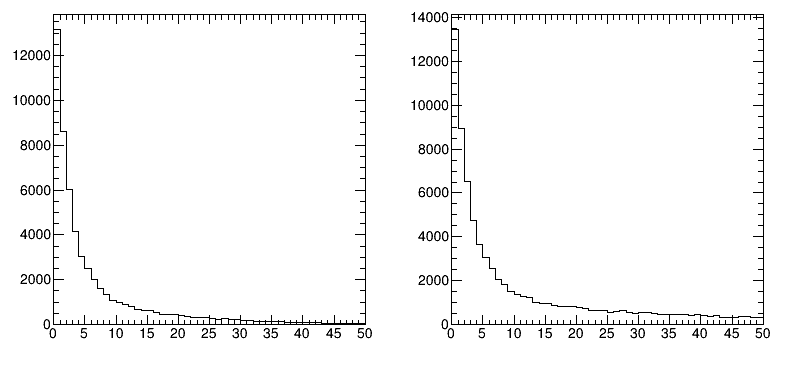
\includegraphics[max size={\textwidth}{\textheight}]{LeptonEfficiencyVsLxyFromMC_files/LeptonEfficiencyVsLxyFromMC_13_0.png}
    \par
    \end{center}
    
            \end{InvisibleVerbatim}
            
        
    


    % Make sure that atleast 4 lines are below the HR
    \needspace{4\baselineskip}

    
        \vspace{6pt}
        \makebox[0.1\linewidth]{\smaller\hfill\tt\color{nbframe-in-prompt}In\hspace{4pt}{[}9{]}:\hspace{4pt}}\\*
        \vspace{-2.65\baselineskip}
        \begin{ColorVerbatim}
            \vspace{-0.7\baselineskip}
            \begin{Verbatim}[commandchars=\\\{\}]
\PY{n}{canvasAndEff} \PY{o}{=} \PY{n}{drawEff}\PY{p}{(}\PY{l+s}{\PYZdq{}}\PY{l+s}{LeptonRecoEfficiencyCanvas}\PY{l+s}{\PYZdq{}}\PY{p}{,} \PY{n}{leptonEffNum}\PY{p}{,} \PY{n}{leptonEffDen}\PY{p}{)}
\PY{n}{canvasAndEff}\PY{p}{[}\PY{l+m+mi}{0}\PY{p}{]}
\end{Verbatim}

            
                \vspace{-0.2\baselineskip}
            
        \end{ColorVerbatim}
    

    

        % If the first block is an image, minipage the image.  Else
        % request a certain amount of space for the input text.
        \needspace{4\baselineskip}
        
        

            % Add document contents.
            
                \makebox[0.1\linewidth]{\smaller\hfill\tt\color{nbframe-out-prompt}Out\hspace{4pt}{[}9{]}:\hspace{4pt}}\\*
                \vspace{-2.55\baselineskip}\begin{InvisibleVerbatim}
                \vspace{-0.5\baselineskip}
    \begin{center}
    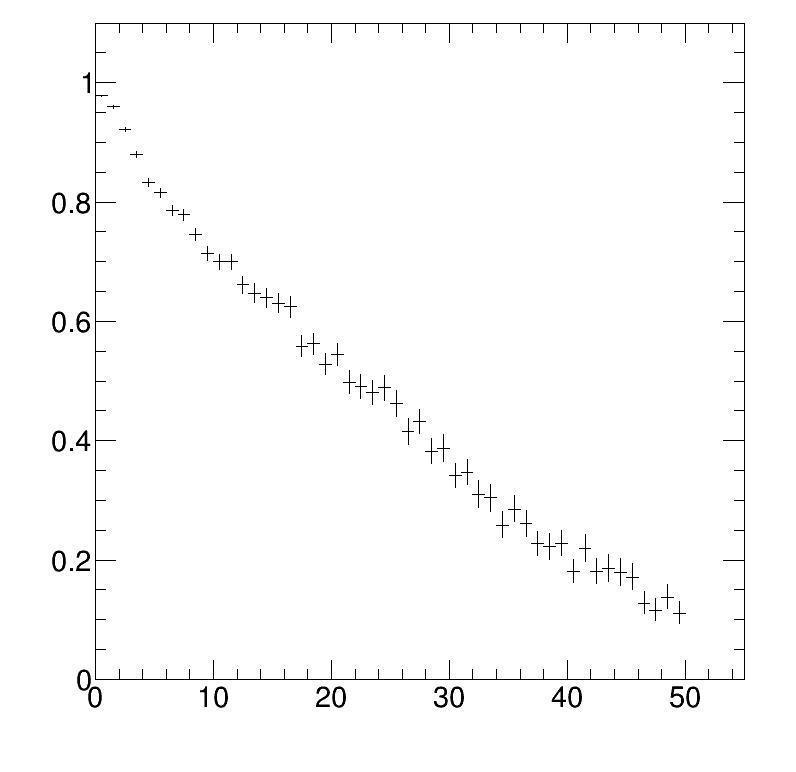
\includegraphics[max size={\textwidth}{\textheight}]{LeptonEfficiencyVsLxyFromMC_files/LeptonEfficiencyVsLxyFromMC_14_0.png}
    \par
    \end{center}
    
            \end{InvisibleVerbatim}
            
        
    
\section{Electrons Lower Pt}

    % Make sure that atleast 4 lines are below the HR
    \needspace{4\baselineskip}

    
        \vspace{6pt}
        \makebox[0.1\linewidth]{\smaller\hfill\tt\color{nbframe-in-prompt}In\hspace{4pt}{[}10{]}:\hspace{4pt}}\\*
        \vspace{-2.65\baselineskip}
        \begin{ColorVerbatim}
            \vspace{-0.7\baselineskip}
            \begin{Verbatim}[commandchars=\\\{\}]
\PY{n}{directory} \PY{o}{=} \PY{n}{inputFile}\PY{o}{.}\PY{n}{Get}\PY{p}{(}\PY{l+s}{\PYZdq{}}\PY{l+s}{eTrackAnalysis}\PY{l+s}{\PYZdq{}}\PY{p}{)}
\PY{n}{tree} \PY{o}{=} \PY{n}{directory}\PY{o}{.}\PY{n}{Get}\PY{p}{(}\PY{l+s}{\PYZdq{}}\PY{l+s}{outputTree}\PY{l+s}{\PYZdq{}}\PY{p}{)}

\PY{n}{chosenPdgId} \PY{o}{=} \PY{l+m+mi}{11}
\PY{c}{\PYZsh{} Acceptance cuts (for electrons)}
\PY{n}{ptCutElecLow} \PY{o}{=} \PY{l+m+mf}{21.}
\PY{n}{etCutElecLow} \PY{o}{=} \PY{l+m+mf}{25.}

\PY{n}{leptonEffNumElecLow} \PY{o}{=} \PY{n}{TH1F}\PY{p}{(}\PY{l+s}{\PYZdq{}}\PY{l+s}{LeptonEffNumElecLow}\PY{l+s}{\PYZdq{}}\PY{p}{,} \PY{l+s}{\PYZdq{}}\PY{l+s}{lepton eff num for lower Et electron}\PY{l+s}{\PYZdq{}}\PY{p}{,} \PY{n}{nBins}\PY{p}{,} \PY{l+m+mi}{0}\PY{p}{,} \PY{l+m+mi}{50}\PY{p}{)}
\PY{n}{leptonEffDenElecLow} \PY{o}{=} \PY{n}{TH1F}\PY{p}{(}\PY{l+s}{\PYZdq{}}\PY{l+s}{LeptonEffDenomElecLow}\PY{l+s}{\PYZdq{}}\PY{p}{,} \PY{l+s}{\PYZdq{}}\PY{l+s}{lepton eff denom for lower Et electron}\PY{l+s}{\PYZdq{}}\PY{p}{,} \PY{n}{nBins}\PY{p}{,} \PY{l+m+mi}{0}\PY{p}{,} \PY{l+m+mi}{50}\PY{p}{)}

\PY{c}{\PYZsh{} num = 0}
\PY{k}{for} \PY{n}{event} \PY{o+ow}{in} \PY{n}{tree}\PY{p}{:}
    \PY{c}{\PYZsh{} num += 1}
    \PY{n}{computeLeptonEff}\PY{p}{(}\PY{n}{event}\PY{o}{.}\PY{n}{candidates}\PY{p}{,} \PY{n}{leptonEffNumElecLow}\PY{p}{,} \PY{n}{leptonEffDenElecLow}\PY{p}{,} \PYZbs{}
                     \PY{n}{chosenPdgId}\PY{p}{,} \PY{n}{signalPdgIds}\PY{p}{,} \PY{n}{ptCutElecLow}\PY{p}{,} \PY{n}{etCutElecLow}\PY{p}{,} \PY{n}{etaCut}\PY{p}{,} \PY{n}{LxyCut}\PY{p}{)}
    \PY{c}{\PYZsh{} if num == 100:}
    \PY{c}{\PYZsh{}     break}
\end{Verbatim}

            
                \vspace{-0.2\baselineskip}
            
        \end{ColorVerbatim}
    


    % Make sure that atleast 4 lines are below the HR
    \needspace{4\baselineskip}

    
        \vspace{6pt}
        \makebox[0.1\linewidth]{\smaller\hfill\tt\color{nbframe-in-prompt}In\hspace{4pt}{[}11{]}:\hspace{4pt}}\\*
        \vspace{-2.65\baselineskip}
        \begin{ColorVerbatim}
            \vspace{-0.7\baselineskip}
            \begin{Verbatim}[commandchars=\\\{\}]
\PY{n}{canvas} \PY{o}{=} \PY{n}{drawCheck}\PY{p}{(}\PY{l+s}{\PYZdq{}}\PY{l+s}{LeptonRecoEfficiencyCheckCanvasElecLow}\PY{l+s}{\PYZdq{}}\PY{p}{,} \PY{n}{leptonEffNumElecLow}\PY{p}{,} \PY{n}{leptonEffDenElecLow}\PY{p}{)}
\PY{n}{canvas}
\end{Verbatim}

            
                \vspace{-0.2\baselineskip}
            
        \end{ColorVerbatim}
    

    

        % If the first block is an image, minipage the image.  Else
        % request a certain amount of space for the input text.
        \needspace{4\baselineskip}
        
        

            % Add document contents.
            
                \makebox[0.1\linewidth]{\smaller\hfill\tt\color{nbframe-out-prompt}Out\hspace{4pt}{[}11{]}:\hspace{4pt}}\\*
                \vspace{-2.55\baselineskip}\begin{InvisibleVerbatim}
                \vspace{-0.5\baselineskip}
    \begin{center}
    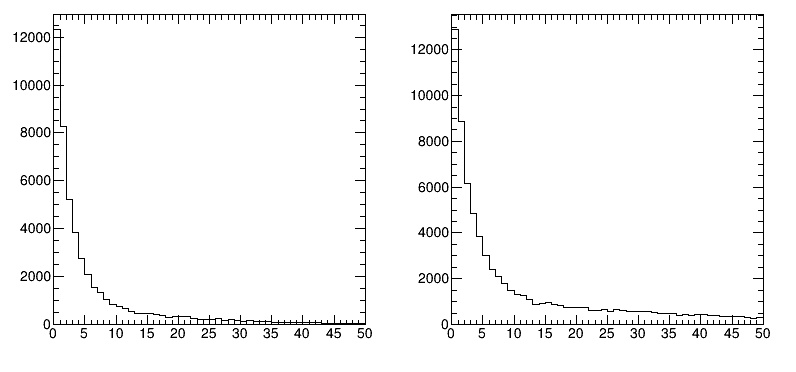
\includegraphics[max size={\textwidth}{\textheight}]{LeptonEfficiencyVsLxyFromMC_files/LeptonEfficiencyVsLxyFromMC_17_0.png}
    \par
    \end{center}
    
            \end{InvisibleVerbatim}
            
        
    


    % Make sure that atleast 4 lines are below the HR
    \needspace{4\baselineskip}

    
        \vspace{6pt}
        \makebox[0.1\linewidth]{\smaller\hfill\tt\color{nbframe-in-prompt}In\hspace{4pt}{[}12{]}:\hspace{4pt}}\\*
        \vspace{-2.65\baselineskip}
        \begin{ColorVerbatim}
            \vspace{-0.7\baselineskip}
            \begin{Verbatim}[commandchars=\\\{\}]
\PY{n}{canvasAndEffElecLow} \PY{o}{=} \PY{n}{drawEff}\PY{p}{(}\PY{l+s}{\PYZdq{}}\PY{l+s}{LeptonRecoEfficiencyCanvasElecLow}\PY{l+s}{\PYZdq{}}\PY{p}{,} \PY{n}{leptonEffNumElecLow}\PY{p}{,} \PY{n}{leptonEffDenElecLow}\PY{p}{)}
\PY{n}{canvasAndEffElecLow}\PY{p}{[}\PY{l+m+mi}{0}\PY{p}{]}
\end{Verbatim}

            
                \vspace{-0.2\baselineskip}
            
        \end{ColorVerbatim}
    

    

        % If the first block is an image, minipage the image.  Else
        % request a certain amount of space for the input text.
        \needspace{4\baselineskip}
        
        

            % Add document contents.
            
                \makebox[0.1\linewidth]{\smaller\hfill\tt\color{nbframe-out-prompt}Out\hspace{4pt}{[}12{]}:\hspace{4pt}}\\*
                \vspace{-2.55\baselineskip}\begin{InvisibleVerbatim}
                \vspace{-0.5\baselineskip}
    \begin{center}
    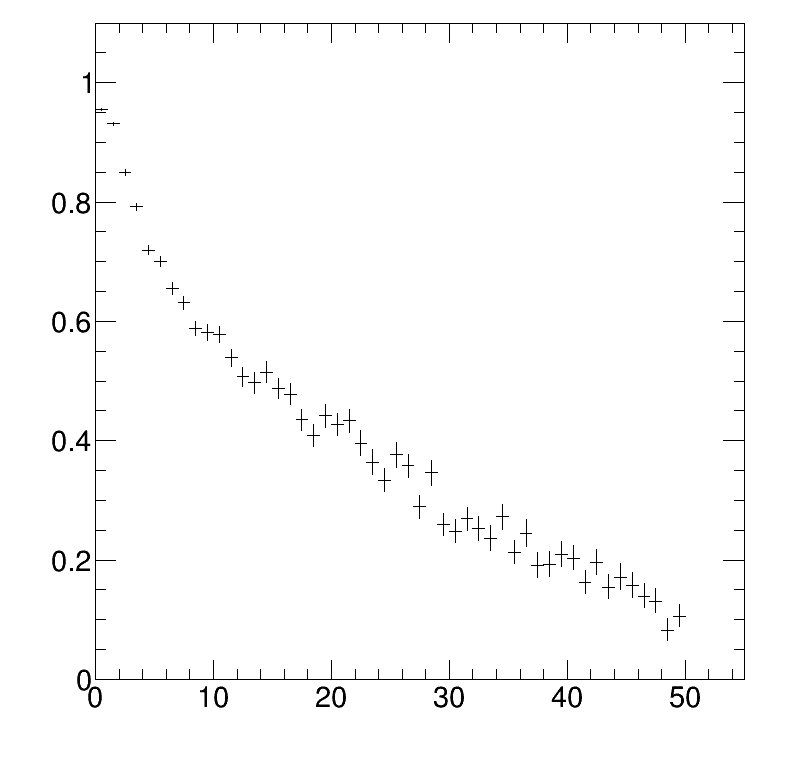
\includegraphics[max size={\textwidth}{\textheight}]{LeptonEfficiencyVsLxyFromMC_files/LeptonEfficiencyVsLxyFromMC_18_0.png}
    \par
    \end{center}
    
            \end{InvisibleVerbatim}
            
        
    
\section{Electrons Higher Pt}

    % Make sure that atleast 4 lines are below the HR
    \needspace{4\baselineskip}

    
        \vspace{6pt}
        \makebox[0.1\linewidth]{\smaller\hfill\tt\color{nbframe-in-prompt}In\hspace{4pt}{[}13{]}:\hspace{4pt}}\\*
        \vspace{-2.65\baselineskip}
        \begin{ColorVerbatim}
            \vspace{-0.7\baselineskip}
            \begin{Verbatim}[commandchars=\\\{\}]
\PY{n}{directory} \PY{o}{=} \PY{n}{inputFile}\PY{o}{.}\PY{n}{Get}\PY{p}{(}\PY{l+s}{\PYZdq{}}\PY{l+s}{eTrackAnalysis}\PY{l+s}{\PYZdq{}}\PY{p}{)}
\PY{n}{tree} \PY{o}{=} \PY{n}{directory}\PY{o}{.}\PY{n}{Get}\PY{p}{(}\PY{l+s}{\PYZdq{}}\PY{l+s}{outputTree}\PY{l+s}{\PYZdq{}}\PY{p}{)}

\PY{n}{chosenPdgId} \PY{o}{=} \PY{l+m+mi}{11}
\PY{c}{\PYZsh{} Acceptance cuts (for electrons)}
\PY{n}{ptCutElecHigh} \PY{o}{=} \PY{l+m+mf}{36.}
\PY{n}{etCutElecHigh} \PY{o}{=} \PY{l+m+mf}{40.}

\PY{n}{leptonEffNumElecHigh} \PY{o}{=} \PY{n}{TH1F}\PY{p}{(}\PY{l+s}{\PYZdq{}}\PY{l+s}{LeptonEffNumElecHigh}\PY{l+s}{\PYZdq{}}\PY{p}{,} \PY{l+s}{\PYZdq{}}\PY{l+s}{lepton eff num for higher Et electron}\PY{l+s}{\PYZdq{}}\PY{p}{,} \PY{n}{nBins}\PY{p}{,} \PY{l+m+mi}{0}\PY{p}{,} \PY{l+m+mi}{50}\PY{p}{)}
\PY{n}{leptonEffDenElecHigh} \PY{o}{=} \PY{n}{TH1F}\PY{p}{(}\PY{l+s}{\PYZdq{}}\PY{l+s}{LeptonEffDenomElecHigh}\PY{l+s}{\PYZdq{}}\PY{p}{,} \PY{l+s}{\PYZdq{}}\PY{l+s}{lepton eff denom for higher Et electron}\PY{l+s}{\PYZdq{}}\PY{p}{,} \PY{n}{nBins}\PY{p}{,} \PY{l+m+mi}{0}\PY{p}{,} \PY{l+m+mi}{50}\PY{p}{)}

\PY{c}{\PYZsh{} num = 0}
\PY{k}{for} \PY{n}{event} \PY{o+ow}{in} \PY{n}{tree}\PY{p}{:}
    \PY{c}{\PYZsh{} num += 1}
    \PY{n}{computeLeptonEff}\PY{p}{(}\PY{n}{event}\PY{o}{.}\PY{n}{candidates}\PY{p}{,} \PY{n}{leptonEffNumElecHigh}\PY{p}{,} \PY{n}{leptonEffDenElecHigh}\PY{p}{,} \PYZbs{}
                     \PY{n}{chosenPdgId}\PY{p}{,} \PY{n}{signalPdgIds}\PY{p}{,} \PY{n}{ptCutElecHigh}\PY{p}{,} \PY{n}{etCutElecHigh}\PY{p}{,} \PY{n}{etaCut}\PY{p}{,} \PY{n}{LxyCut}\PY{p}{)}
    \PY{c}{\PYZsh{} if num == 100:}
    \PY{c}{\PYZsh{}     break}
\end{Verbatim}

            
                \vspace{-0.2\baselineskip}
            
        \end{ColorVerbatim}
    


    % Make sure that atleast 4 lines are below the HR
    \needspace{4\baselineskip}

    
        \vspace{6pt}
        \makebox[0.1\linewidth]{\smaller\hfill\tt\color{nbframe-in-prompt}In\hspace{4pt}{[}14{]}:\hspace{4pt}}\\*
        \vspace{-2.65\baselineskip}
        \begin{ColorVerbatim}
            \vspace{-0.7\baselineskip}
            \begin{Verbatim}[commandchars=\\\{\}]
\PY{n}{canvas} \PY{o}{=} \PY{n}{drawCheck}\PY{p}{(}\PY{l+s}{\PYZdq{}}\PY{l+s}{LeptonRecoEfficiencyCheckCanvasElecHigh}\PY{l+s}{\PYZdq{}}\PY{p}{,} \PY{n}{leptonEffNumElecHigh}\PY{p}{,} \PY{n}{leptonEffDenElecHigh}\PY{p}{)}
\PY{n}{canvas}
\end{Verbatim}

            
                \vspace{-0.2\baselineskip}
            
        \end{ColorVerbatim}
    

    

        % If the first block is an image, minipage the image.  Else
        % request a certain amount of space for the input text.
        \needspace{4\baselineskip}
        
        

            % Add document contents.
            
                \makebox[0.1\linewidth]{\smaller\hfill\tt\color{nbframe-out-prompt}Out\hspace{4pt}{[}14{]}:\hspace{4pt}}\\*
                \vspace{-2.55\baselineskip}\begin{InvisibleVerbatim}
                \vspace{-0.5\baselineskip}
    \begin{center}
    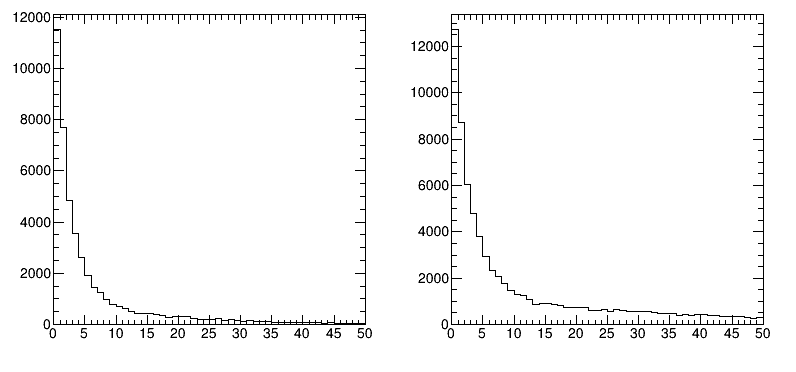
\includegraphics[max size={\textwidth}{\textheight}]{LeptonEfficiencyVsLxyFromMC_files/LeptonEfficiencyVsLxyFromMC_21_0.png}
    \par
    \end{center}
    
            \end{InvisibleVerbatim}
            
        
    


    % Make sure that atleast 4 lines are below the HR
    \needspace{4\baselineskip}

    
        \vspace{6pt}
        \makebox[0.1\linewidth]{\smaller\hfill\tt\color{nbframe-in-prompt}In\hspace{4pt}{[}15{]}:\hspace{4pt}}\\*
        \vspace{-2.65\baselineskip}
        \begin{ColorVerbatim}
            \vspace{-0.7\baselineskip}
            \begin{Verbatim}[commandchars=\\\{\}]
\PY{n}{canvasAndEffElecHigh} \PY{o}{=} \PY{n}{drawEff}\PY{p}{(}\PY{l+s}{\PYZdq{}}\PY{l+s}{LeptonRecoEfficiencyCanvasElecHigh}\PY{l+s}{\PYZdq{}}\PY{p}{,} \PY{n}{leptonEffNumElecHigh}\PY{p}{,} \PY{n}{leptonEffDenElecHigh}\PY{p}{)}
\PY{n}{canvasAndEffElecHigh}\PY{p}{[}\PY{l+m+mi}{0}\PY{p}{]}
\end{Verbatim}

            
                \vspace{-0.2\baselineskip}
            
        \end{ColorVerbatim}
    

    

        % If the first block is an image, minipage the image.  Else
        % request a certain amount of space for the input text.
        \needspace{4\baselineskip}
        
        

            % Add document contents.
            
                \makebox[0.1\linewidth]{\smaller\hfill\tt\color{nbframe-out-prompt}Out\hspace{4pt}{[}15{]}:\hspace{4pt}}\\*
                \vspace{-2.55\baselineskip}\begin{InvisibleVerbatim}
                \vspace{-0.5\baselineskip}
    \begin{center}
    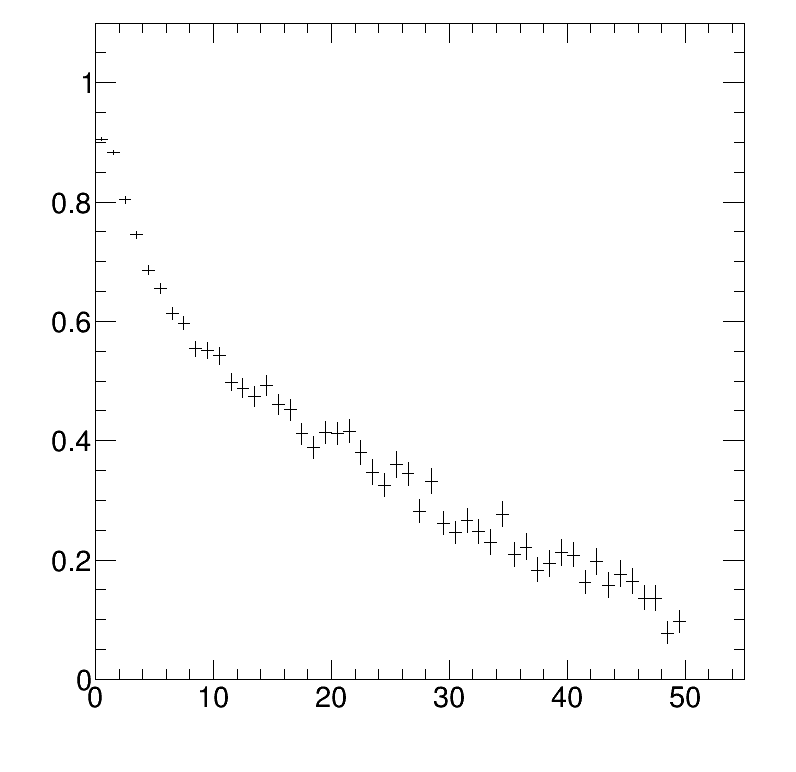
\includegraphics[max size={\textwidth}{\textheight}]{LeptonEfficiencyVsLxyFromMC_files/LeptonEfficiencyVsLxyFromMC_22_0.png}
    \par
    \end{center}
    
            \end{InvisibleVerbatim}
            
        
    
\section{Overlay of all efficiencies}

    % Make sure that atleast 4 lines are below the HR
    \needspace{4\baselineskip}

    
        \vspace{6pt}
        \makebox[0.1\linewidth]{\smaller\hfill\tt\color{nbframe-in-prompt}In\hspace{4pt}{[}87{]}:\hspace{4pt}}\\*
        \vspace{-2.65\baselineskip}
        \begin{ColorVerbatim}
            \vspace{-0.7\baselineskip}
            \begin{Verbatim}[commandchars=\\\{\}]
\PY{n}{leptonEffOverlayCanvas} \PY{o}{=} \PY{n}{rootnotes}\PY{o}{.}\PY{n}{canvas}\PY{p}{(}\PY{l+s}{\PYZdq{}}\PY{l+s}{LeptonEffOverlay}\PY{l+s}{\PYZdq{}}\PY{p}{,} \PY{p}{(}\PY{l+m+mi}{800}\PY{p}{,} \PY{l+m+mi}{800}\PY{p}{)}\PY{p}{)}
\PY{n}{canvasAndEff}\PY{p}{[}\PY{l+m+mi}{1}\PY{p}{]}\PY{o}{.}\PY{n}{Draw}\PY{p}{(}\PY{p}{)}
\PY{c}{\PYZsh{} canvasAndEff[1].GetPaintedGraph().GetXaxis().SetTitle(\PYZdq{}L\PYZus{}\PYZob{}xy\PYZcb{} [cm]\PYZdq{})}
\PY{c}{\PYZsh{} canvasAndEff[1].GetPaintedGraph().GetYaxis().SetTitle(\PYZdq{}Tracking Efficiency\PYZdq{})}
\PY{n}{canvasAndEff}\PY{p}{[}\PY{l+m+mi}{1}\PY{p}{]}\PY{o}{.}\PY{n}{SetTitle}\PY{p}{(}\PY{l+s}{\PYZdq{}}\PY{l+s}{myTitle; L\PYZus{}\PYZob{}xy\PYZcb{} [cm] ; Tracking Efficiency}\PY{l+s}{\PYZdq{}}\PY{p}{)}\PY{p}{;} 
\PY{n}{ROOT}\PY{o}{.}\PY{n}{gPad}\PY{o}{.}\PY{n}{Update}\PY{p}{(}\PY{p}{)}
\PY{n}{canvasAndEffElecLow}\PY{p}{[}\PY{l+m+mi}{1}\PY{p}{]}\PY{o}{.}\PY{n}{Draw}\PY{p}{(}\PY{l+s}{\PYZdq{}}\PY{l+s}{same}\PY{l+s}{\PYZdq{}}\PY{p}{)}
\PY{n}{canvasAndEffElecLow}\PY{p}{[}\PY{l+m+mi}{1}\PY{p}{]}\PY{o}{.}\PY{n}{SetLineColor}\PY{p}{(}\PY{l+m+mi}{2}\PY{p}{)}
\PY{n}{canvasAndEffElecHigh}\PY{p}{[}\PY{l+m+mi}{1}\PY{p}{]}\PY{o}{.}\PY{n}{Draw}\PY{p}{(}\PY{l+s}{\PYZdq{}}\PY{l+s}{same}\PY{l+s}{\PYZdq{}}\PY{p}{)}
\PY{n}{canvasAndEffElecHigh}\PY{p}{[}\PY{l+m+mi}{1}\PY{p}{]}\PY{o}{.}\PY{n}{SetLineColor}\PY{p}{(}\PY{l+m+mi}{4}\PY{p}{)}
\PY{n}{legend} \PY{o}{=} \PY{n}{TLegend}\PY{p}{(}\PY{l+m+mf}{0.45}\PY{p}{,}\PY{l+m+mf}{0.7}\PY{p}{,}\PY{l+m+mf}{0.85}\PY{p}{,}\PY{l+m+mf}{0.9}\PY{p}{)}
\PY{n}{legend}\PY{o}{.}\PY{n}{AddEntry}\PY{p}{(}\PY{n}{canvasAndEff}\PY{p}{[}\PY{l+m+mi}{1}\PY{p}{]}\PY{p}{,} \PY{l+s}{\PYZdq{}}\PY{l+s}{Muon Efficiency}\PY{l+s}{\PYZdq{}}\PY{p}{,} \PY{l+s}{\PYZdq{}}\PY{l+s}{l}\PY{l+s}{\PYZdq{}}\PY{p}{)}
\PY{n}{legend}\PY{o}{.}\PY{n}{AddEntry}\PY{p}{(}\PY{n}{canvasAndEffElecLow}\PY{p}{[}\PY{l+m+mi}{1}\PY{p}{]}\PY{p}{,} \PY{l+s}{\PYZdq{}}\PY{l+s}{Low E\PYZus{}\PYZob{}T\PYZcb{} electron Efficiency}\PY{l+s}{\PYZdq{}}\PY{p}{,} \PY{l+s}{\PYZdq{}}\PY{l+s}{l}\PY{l+s}{\PYZdq{}}\PY{p}{)}
\PY{n}{legend}\PY{o}{.}\PY{n}{AddEntry}\PY{p}{(}\PY{n}{canvasAndEffElecHigh}\PY{p}{[}\PY{l+m+mi}{1}\PY{p}{]}\PY{p}{,} \PY{l+s}{\PYZdq{}}\PY{l+s}{High E\PYZus{}\PYZob{}T\PYZcb{} electron Efficiency}\PY{l+s}{\PYZdq{}}\PY{p}{,} \PY{l+s}{\PYZdq{}}\PY{l+s}{l}\PY{l+s}{\PYZdq{}}\PY{p}{)}
\PY{n}{legend}\PY{o}{.}\PY{n}{SetFillColor}\PY{p}{(}\PY{l+m+mi}{0}\PY{p}{)}
\PY{n}{legend}\PY{o}{.}\PY{n}{SetLineColor}\PY{p}{(}\PY{l+m+mi}{0}\PY{p}{)}
\PY{n}{legend}\PY{o}{.}\PY{n}{Draw}\PY{p}{(}\PY{l+s}{\PYZdq{}}\PY{l+s}{same}\PY{l+s}{\PYZdq{}}\PY{p}{)}
\PY{n}{leptonEffOverlayCanvas}
\PY{c}{\PYZsh{} leptonEffOverlayCanvas.SaveAs(\PYZdq{}leptonEffOverlay.pdf\PYZdq{})}
\end{Verbatim}

            
                \vspace{-0.2\baselineskip}
            
        \end{ColorVerbatim}
    

    

        % If the first block is an image, minipage the image.  Else
        % request a certain amount of space for the input text.
        \needspace{4\baselineskip}
        
        

            % Add document contents.
            
                \begin{InvisibleVerbatim}
                \vspace{-0.5\baselineskip}
\begin{alltt}TCanvas::Constructor:0: RuntimeWarning: Deleting canvas with same
name: LeptonEffOverlay
\end{alltt}

            \end{InvisibleVerbatim}
            
                \makebox[0.1\linewidth]{\smaller\hfill\tt\color{nbframe-out-prompt}Out\hspace{4pt}{[}87{]}:\hspace{4pt}}\\*
                \vspace{-2.55\baselineskip}\begin{InvisibleVerbatim}
                \vspace{-0.5\baselineskip}
    \begin{center}
    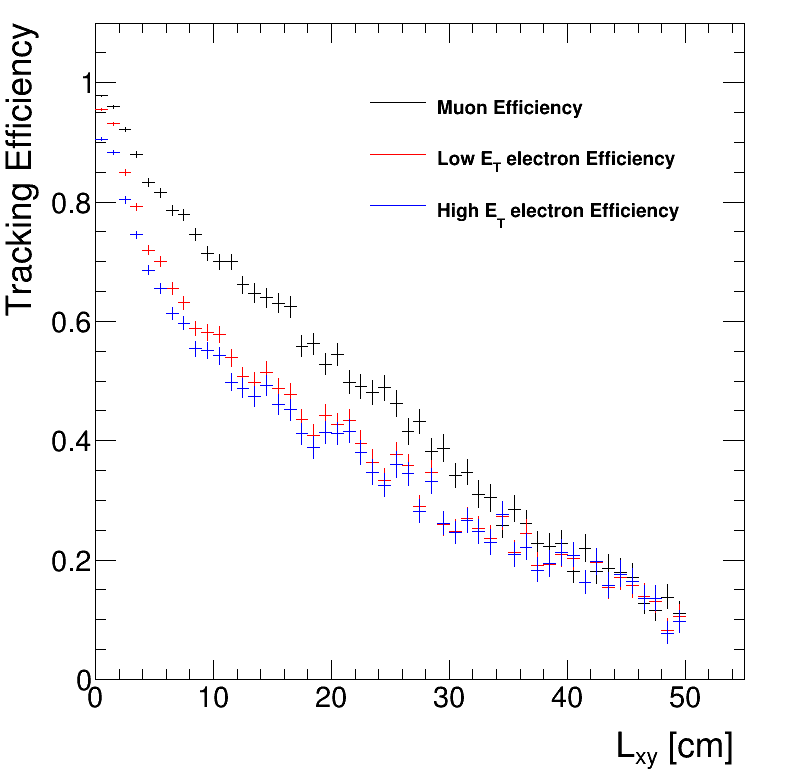
\includegraphics[max size={\textwidth}{\textheight}]{LeptonEfficiencyVsLxyFromMC_files/LeptonEfficiencyVsLxyFromMC_24_1.png}
    \par
    \end{center}
    
            \end{InvisibleVerbatim}
            
        
    
Print the maximum difference between muon and electron low and high
efficiencies

    % Make sure that atleast 4 lines are below the HR
    \needspace{4\baselineskip}

    
        \vspace{6pt}
        \makebox[0.1\linewidth]{\smaller\hfill\tt\color{nbframe-in-prompt}In\hspace{4pt}{[}91{]}:\hspace{4pt}}\\*
        \vspace{-2.65\baselineskip}
        \begin{ColorVerbatim}
            \vspace{-0.7\baselineskip}
            \begin{Verbatim}[commandchars=\\\{\}]
\PY{n}{muEffMaxDiff} \PY{o}{=} \PY{l+m+mi}{0}

\PY{k}{for} \PY{n}{i} \PY{o+ow}{in} \PY{n+nb}{range}\PY{p}{(}\PY{l+m+mi}{1}\PY{p}{,} \PY{n}{nBins}\PY{o}{+}\PY{l+m+mi}{1}\PY{p}{)}\PY{p}{:}
    \PY{n}{muEff} \PY{o}{=} \PY{n}{canvasAndEff}\PY{p}{[}\PY{l+m+mi}{1}\PY{p}{]}\PY{o}{.}\PY{n}{GetEfficiency}\PY{p}{(}\PY{n}{i}\PY{p}{)}
    \PY{n}{diff} \PY{o}{=} \PY{n+nb}{max}\PY{p}{(} \PY{n+nb}{abs}\PY{p}{(}\PY{n}{muEff} \PY{o}{\PYZhy{}} \PY{n}{canvasAndEffElecLow}\PY{p}{[}\PY{l+m+mi}{1}\PY{p}{]}\PY{o}{.}\PY{n}{GetEfficiency}\PY{p}{(}\PY{n}{i}\PY{p}{)}\PY{p}{)}\PY{p}{,} \PYZbs{}
                \PY{n+nb}{abs}\PY{p}{(}\PY{n}{muEff} \PY{o}{\PYZhy{}} \PY{n}{canvasAndEffElecHigh}\PY{p}{[}\PY{l+m+mi}{1}\PY{p}{]}\PY{o}{.}\PY{n}{GetEfficiency}\PY{p}{(}\PY{n}{i}\PY{p}{)}\PY{p}{)} \PY{p}{)}
    \PY{k}{if} \PY{n}{diff} \PY{o}{\PYZgt{}} \PY{n}{muEffMaxDiff}\PY{p}{:}
        \PY{n}{muEffMaxDiff} \PY{o}{=} \PY{n}{diff}

\PY{k}{print} \PY{n}{muEffMaxDiff}
\end{Verbatim}

            
                \vspace{-0.2\baselineskip}
            
        \end{ColorVerbatim}
    

    

        % If the first block is an image, minipage the image.  Else
        % request a certain amount of space for the input text.
        \needspace{4\baselineskip}
        
        

            % Add document contents.
            
                \begin{InvisibleVerbatim}
                \vspace{-0.5\baselineskip}
\begin{alltt}0.201467855628
\end{alltt}

            \end{InvisibleVerbatim}
            
        
    
The electron systematic can be written as:

$e_{syst} = \mu_{syst} + k\cdot (\epsilon_{\mu_{MC}} - \epsilon_{e_{MC}})$

where, $e_{syst} = \epsilon_{e_{Data}} - \epsilon_{e_{MC}}$, and the
same for muons. And $\epsilon$ represents the efficiency.

Assuming an uncertainty on the material of 10\% ($k = 0.1$), the
possible additional variation of the data-MC efficiency difference for
electrons is:

    % Make sure that atleast 4 lines are below the HR
    \needspace{4\baselineskip}

    
        \vspace{6pt}
        \makebox[0.1\linewidth]{\smaller\hfill\tt\color{nbframe-in-prompt}In\hspace{4pt}{[}76{]}:\hspace{4pt}}\\*
        \vspace{-2.65\baselineskip}
        \begin{ColorVerbatim}
            \vspace{-0.7\baselineskip}
            \begin{Verbatim}[commandchars=\\\{\}]
\PY{n}{materialSyst} \PY{o}{=} \PY{n}{maxDiff}\PY{o}{*}\PY{l+m+mf}{0.1}
\PY{n}{materialSyst}
\end{Verbatim}

            
                \vspace{-0.2\baselineskip}
            
        \end{ColorVerbatim}
    

    

        % If the first block is an image, minipage the image.  Else
        % request a certain amount of space for the input text.
        \needspace{4\baselineskip}
        
        

            % Add document contents.
            
                \makebox[0.1\linewidth]{\smaller\hfill\tt\color{nbframe-out-prompt}Out\hspace{4pt}{[}76{]}:\hspace{4pt}}\\*
                \vspace{-2.55\baselineskip}\begin{InvisibleVerbatim}
                \vspace{-0.5\baselineskip}
\begin{alltt}0.020146785562804227\end{alltt}

            \end{InvisibleVerbatim}
            
        
    
Doubling this for a dilepton systematic leads to

    % Make sure that atleast 4 lines are below the HR
    \needspace{4\baselineskip}

    
        \vspace{6pt}
        \makebox[0.1\linewidth]{\smaller\hfill\tt\color{nbframe-in-prompt}In\hspace{4pt}{[}77{]}:\hspace{4pt}}\\*
        \vspace{-2.65\baselineskip}
        \begin{ColorVerbatim}
            \vspace{-0.7\baselineskip}
            \begin{Verbatim}[commandchars=\\\{\}]
\PY{n}{materialSyst}\PY{o}{*}\PY{l+m+mi}{2}
\end{Verbatim}

            
                \vspace{-0.2\baselineskip}
            
        \end{ColorVerbatim}
    

    

        % If the first block is an image, minipage the image.  Else
        % request a certain amount of space for the input text.
        \needspace{4\baselineskip}
        
        

            % Add document contents.
            
                \makebox[0.1\linewidth]{\smaller\hfill\tt\color{nbframe-out-prompt}Out\hspace{4pt}{[}77{]}:\hspace{4pt}}\\*
                \vspace{-2.55\baselineskip}\begin{InvisibleVerbatim}
                \vspace{-0.5\baselineskip}
\begin{alltt}0.040293571125608454\end{alltt}

            \end{InvisibleVerbatim}
            
        
    
From the tracking systematics in the paper

\begin{itemize}
\itemsep1pt\parskip0pt\parsep0pt
\item
  6.1\% from cosmics
\item
  9.8\% from track embedding
\end{itemize}

We get:

    % Make sure that atleast 4 lines are below the HR
    \needspace{4\baselineskip}

    
        \vspace{6pt}
        \makebox[0.1\linewidth]{\smaller\hfill\tt\color{nbframe-in-prompt}In\hspace{4pt}{[}78{]}:\hspace{4pt}}\\*
        \vspace{-2.65\baselineskip}
        \begin{ColorVerbatim}
            \vspace{-0.7\baselineskip}
            \begin{Verbatim}[commandchars=\\\{\}]
\PY{n}{totalSystWithoutMaterial} \PY{o}{=} \PY{n}{ROOT}\PY{o}{.}\PY{n}{Math}\PY{o}{.}\PY{n}{sqrt}\PY{p}{(}\PY{l+m+mf}{0.061}\PY{o}{*}\PY{o}{*}\PY{l+m+mi}{2} \PY{o}{+} \PY{l+m+mf}{0.098}\PY{o}{*}\PY{o}{*}\PY{l+m+mi}{2}\PY{p}{)}
\PY{n}{totalSystWithoutMaterial}
\end{Verbatim}

            
                \vspace{-0.2\baselineskip}
            
        \end{ColorVerbatim}
    

    

        % If the first block is an image, minipage the image.  Else
        % request a certain amount of space for the input text.
        \needspace{4\baselineskip}
        
        

            % Add document contents.
            
                \makebox[0.1\linewidth]{\smaller\hfill\tt\color{nbframe-out-prompt}Out\hspace{4pt}{[}78{]}:\hspace{4pt}}\\*
                \vspace{-2.55\baselineskip}\begin{InvisibleVerbatim}
                \vspace{-0.5\baselineskip}
\begin{alltt}0.11543396380615197\end{alltt}

            \end{InvisibleVerbatim}
            
        
    
Adding the material systematic for electrons yields:

    % Make sure that atleast 4 lines are below the HR
    \needspace{4\baselineskip}

    
        \vspace{6pt}
        \makebox[0.1\linewidth]{\smaller\hfill\tt\color{nbframe-in-prompt}In\hspace{4pt}{[}79{]}:\hspace{4pt}}\\*
        \vspace{-2.65\baselineskip}
        \begin{ColorVerbatim}
            \vspace{-0.7\baselineskip}
            \begin{Verbatim}[commandchars=\\\{\}]
\PY{n}{totalSystWithMaterial} \PY{o}{=} \PY{n}{ROOT}\PY{o}{.}\PY{n}{Math}\PY{o}{.}\PY{n}{sqrt}\PY{p}{(}\PY{l+m+mf}{0.061}\PY{o}{*}\PY{o}{*}\PY{l+m+mi}{2} \PY{o}{+} \PY{l+m+mf}{0.098}\PY{o}{*}\PY{o}{*}\PY{l+m+mi}{2} \PY{o}{+} \PY{p}{(}\PY{n}{materialSyst}\PY{o}{*}\PY{l+m+mi}{2}\PY{p}{)}\PY{o}{*}\PY{o}{*}\PY{l+m+mi}{2}\PY{p}{)}
\PY{n}{totalSystWithMaterial}
\end{Verbatim}

            
                \vspace{-0.2\baselineskip}
            
        \end{ColorVerbatim}
    

    

        % If the first block is an image, minipage the image.  Else
        % request a certain amount of space for the input text.
        \needspace{4\baselineskip}
        
        

            % Add document contents.
            
                \makebox[0.1\linewidth]{\smaller\hfill\tt\color{nbframe-out-prompt}Out\hspace{4pt}{[}79{]}:\hspace{4pt}}\\*
                \vspace{-2.55\baselineskip}\begin{InvisibleVerbatim}
                \vspace{-0.5\baselineskip}
\begin{alltt}0.12226435242561287\end{alltt}

            \end{InvisibleVerbatim}
            
        
    
The variation of the systematic is small, keeping two digits will not
change the value from 12\%. The relative variation of the systematic is:

    % Make sure that atleast 4 lines are below the HR
    \needspace{4\baselineskip}

    
        \vspace{6pt}
        \makebox[0.1\linewidth]{\smaller\hfill\tt\color{nbframe-in-prompt}In\hspace{4pt}{[}80{]}:\hspace{4pt}}\\*
        \vspace{-2.65\baselineskip}
        \begin{ColorVerbatim}
            \vspace{-0.7\baselineskip}
            \begin{Verbatim}[commandchars=\\\{\}]
\PY{p}{(}\PY{n}{totalSystWithMaterial} \PY{o}{\PYZhy{}} \PY{n}{totalSystWithoutMaterial}\PY{p}{)}\PY{o}{/}\PY{n}{totalSystWithoutMaterial}
\end{Verbatim}

            
                \vspace{-0.2\baselineskip}
            
        \end{ColorVerbatim}
    

    

        % If the first block is an image, minipage the image.  Else
        % request a certain amount of space for the input text.
        \needspace{4\baselineskip}
        
        

            % Add document contents.
            
                \makebox[0.1\linewidth]{\smaller\hfill\tt\color{nbframe-out-prompt}Out\hspace{4pt}{[}80{]}:\hspace{4pt}}\\*
                \vspace{-2.55\baselineskip}\begin{InvisibleVerbatim}
                \vspace{-0.5\baselineskip}
\begin{alltt}0.059171394572668096\end{alltt}

            \end{InvisibleVerbatim}
            
        
    
\section{Computing the systematic uncertainty for electrons}Definitions:

\begin{itemize}
\itemsep1pt\parskip0pt\parsep0pt
\item
  $\mu_{syst} = \frac{\epsilon_{\mu}^{Data} - \epsilon_{\mu}^{MC}}{\epsilon_{\mu}^{MC}}$
\item
  $e_{syst} = \frac{\epsilon_{e}^{Data} - \epsilon_{e}^{MC}}{\epsilon_{e}^{MC}}$
\end{itemize}

\textbf{Assumption 1}: The difference between electrons and muons is
determined (to first order) by the material.

\textbf{Assumption 2}: The systematic on the tracking efficiency does
not depend on the efficiency. This means that muon and electron
systematics will be the same if material effects are perfectly described
in the simulation even though the efficiency values can be different.

Note that assumption 2 is likely false. However, if the systematic
increases as a function of the efficiency, and because the muon tracking
efficiency is generally higher than the one for electrons, this
assumption would lead to an overestimate of the systematic for
electrons.

We define $a$ as the relative difference of the efficiency for electrons
and muons:

$a = \frac{\epsilon_{\mu} - \epsilon_{e}}{\epsilon_{\mu}}$

then

$\epsilon_{e} = \epsilon_{\mu}\cdot(1 - a)$

and the relative variation of $a$ between data and MC, which from
assumption 1 depends only on the material, is

$k = \frac{a^{MC} - a^{Data}}{a_{MC}}$.

We can compute $a^{MC}$ from our MC efficiencies and $k$ is constrained
by the uncertainty on the material (10\%).

We want to express the systematic on electrons as a function of the
systematic on muons using $k$ and $a^{MC}$.

From the definition of systematic we can write

$e_{syst} = \frac{\epsilon_{e}^{Data} - \epsilon_{e}^{MC}}{\epsilon_{e}^{MC}} = \frac{(1-a^{Data})\cdot\epsilon_{\mu}^{Data} - (1-a^{MC})\cdot\epsilon_{\mu}^{MC}}{(1-a^{MC})\cdot\epsilon_{\mu}^{MC}}$

By adding and subtracting $a^{MC}\cdot\epsilon_{\mu}^{Data}$ at the
numerator we get

$e_{syst} = \mu_{syst} + \frac{a^{MC} - a^{Data}}{1 - a^{MC}}\cdot\frac{\epsilon_{\mu}^{Data}}{\epsilon_{\mu}^{MC}}$

Using the fact that
$\frac{\epsilon_{\mu}^{Data}}{\epsilon_{\mu}^{MC}} = \mu_{syst} + 1$ and
that $a^{MC} - a^{Data} = k\cdot a^{MC}$ we get

$e_{syst} = \mu_{syst} + \frac{k\cdot a^{MC}}{1 - a^{MC}}\cdot(1 + \mu_{syst})$

We compute this systematic below.Maximum relative difference between muons and electrons efficiency in MC
($a^{MC}$):

    % Make sure that atleast 4 lines are below the HR
    \needspace{4\baselineskip}

    
        \vspace{6pt}
        \makebox[0.1\linewidth]{\smaller\hfill\tt\color{nbframe-in-prompt}In\hspace{4pt}{[}122{]}:\hspace{4pt}}\\*
        \vspace{-2.65\baselineskip}
        \begin{ColorVerbatim}
            \vspace{-0.7\baselineskip}
            \begin{Verbatim}[commandchars=\\\{\}]
\PY{n}{effMaxRelDiff} \PY{o}{=} \PY{l+m+mi}{0}

\PY{k}{for} \PY{n}{i} \PY{o+ow}{in} \PY{n+nb}{range}\PY{p}{(}\PY{l+m+mi}{1}\PY{p}{,} \PY{n}{nBins}\PY{o}{+}\PY{l+m+mi}{1}\PY{p}{)}\PY{p}{:}
    \PY{n}{muEff} \PY{o}{=} \PY{n}{canvasAndEff}\PY{p}{[}\PY{l+m+mi}{1}\PY{p}{]}\PY{o}{.}\PY{n}{GetEfficiency}\PY{p}{(}\PY{n}{i}\PY{p}{)}
    \PY{n}{diff} \PY{o}{=} \PY{n+nb}{max}\PY{p}{(} \PY{n+nb}{abs}\PY{p}{(}\PY{n}{muEff} \PY{o}{\PYZhy{}} \PY{n}{canvasAndEffElecLow}\PY{p}{[}\PY{l+m+mi}{1}\PY{p}{]}\PY{o}{.}\PY{n}{GetEfficiency}\PY{p}{(}\PY{n}{i}\PY{p}{)}\PY{p}{)}\PY{o}{/}\PY{n}{muEff}\PY{p}{,} \PYZbs{}
                \PY{n+nb}{abs}\PY{p}{(}\PY{n}{muEff} \PY{o}{\PYZhy{}} \PY{n}{canvasAndEffElecHigh}\PY{p}{[}\PY{l+m+mi}{1}\PY{p}{]}\PY{o}{.}\PY{n}{GetEfficiency}\PY{p}{(}\PY{n}{i}\PY{p}{)}\PY{p}{)}\PY{o}{/}\PY{n}{muEff} \PY{p}{)}
    \PY{k}{if} \PY{n}{diff} \PY{o}{\PYZgt{}} \PY{n}{muEffmaxDiff}\PY{p}{:}
        \PY{n}{effMaxRelDiff} \PY{o}{=} \PY{n}{diff}

\PY{k}{print} \PY{n}{effMaxRelDiff}
\end{Verbatim}

            
                \vspace{-0.2\baselineskip}
            
        \end{ColorVerbatim}
    

    

        % If the first block is an image, minipage the image.  Else
        % request a certain amount of space for the input text.
        \needspace{4\baselineskip}
        
        

            % Add document contents.
            
                \begin{InvisibleVerbatim}
                \vspace{-0.5\baselineskip}
\begin{alltt}0.132016632017
\end{alltt}

            \end{InvisibleVerbatim}
            
        
    
From which we can derive the electron systematic as a function of
$\mu_{syst}$, $a^{MC}$ and $k$:

    % Make sure that atleast 4 lines are below the HR
    \needspace{4\baselineskip}

    
        \vspace{6pt}
        \makebox[0.1\linewidth]{\smaller\hfill\tt\color{nbframe-in-prompt}In\hspace{4pt}{[}123{]}:\hspace{4pt}}\\*
        \vspace{-2.65\baselineskip}
        \begin{ColorVerbatim}
            \vspace{-0.7\baselineskip}
            \begin{Verbatim}[commandchars=\\\{\}]
\PY{n}{muSyst} \PY{o}{=} \PY{n}{ROOT}\PY{o}{.}\PY{n}{Math}\PY{o}{.}\PY{n}{sqrt}\PY{p}{(}\PY{l+m+mf}{0.061}\PY{o}{*}\PY{o}{*}\PY{l+m+mi}{2} \PY{o}{+} \PY{l+m+mf}{0.098}\PY{o}{*}\PY{o}{*}\PY{l+m+mi}{2}\PY{p}{)}
\PY{n}{k} \PY{o}{=} \PY{l+m+mf}{0.1}
\PY{n}{materialTerm} \PY{o}{=} \PY{n}{k}\PY{o}{*}\PY{n}{effMaxRelDiff}\PY{o}{/}\PY{p}{(}\PY{l+m+mi}{1}\PY{o}{\PYZhy{}}\PY{n}{effMaxRelDiff}\PY{p}{)}
\PY{n}{eSyst} \PY{o}{=} \PY{n}{muSyst} \PY{o}{+} \PY{n}{materialTerm}\PY{o}{*}\PY{p}{(}\PY{l+m+mi}{1}\PY{o}{+}\PY{n}{muSyst}\PY{p}{)}
\PY{n}{eSyst}
\end{Verbatim}

            
                \vspace{-0.2\baselineskip}
            
        \end{ColorVerbatim}
    

    

        % If the first block is an image, minipage the image.  Else
        % request a certain amount of space for the input text.
        \needspace{4\baselineskip}
        
        

            % Add document contents.
            
                \makebox[0.1\linewidth]{\smaller\hfill\tt\color{nbframe-out-prompt}Out\hspace{4pt}{[}123{]}:\hspace{4pt}}\\*
                \vspace{-2.55\baselineskip}\begin{InvisibleVerbatim}
                \vspace{-0.5\baselineskip}
\begin{alltt}0.13239924684847307\end{alltt}

            \end{InvisibleVerbatim}
            
        
    
This is \textasciitilde{}1\% bigger than $\mu_{syst}$.

    % Make sure that atleast 4 lines are below the HR
    \needspace{4\baselineskip}

    
        \vspace{6pt}
        \makebox[0.1\linewidth]{\smaller\hfill\tt\color{nbframe-in-prompt}In\hspace{4pt}{[}{]}:\hspace{4pt}}\\*
        \vspace{-2.65\baselineskip}
        \begin{ColorVerbatim}
            \vspace{-0.7\baselineskip}
            \begin{Verbatim}[commandchars=\\\{\}]

\end{Verbatim}

            
                \vspace{0.3\baselineskip}
            
        \end{ColorVerbatim}
    

        

        \renewcommand{\indexname}{Index}
        \printindex

    % End of document
    \end{document}


